\chapter{Evaluation: Blockchain and Games}

Besides the technical possibilities that result from inventions such as Ethereum, what they are useful for is questionable.
The blockchain was initially designed to solve the problems of digital money proposed earlier. 
Ethereum then created a blockchain that could execute Turing-complete code instead of simple operation codes.
According to the Ethereum whitepaper, the use case is that decentralized apps or organizations could be built using smart contracts.
However, are these apps decentralized? What are the benefits or drawbacks? 

\section{Difference between Bitcoin and Ethereum}
Although Ethereum is also based on a blockchain, Bitcoin has critical differences. \cite{Arslanian2022}
Some of them lead to the question: Is Ethereum decentralized?
This chapter will first show the differences and afterward present some arguments for and against Ethereum.

First, there are technical differences.
Besides the fact that Ethereum can run Turing-complete smart contracts, it also has a much shorter block time of only 17 seconds compared to Bitcoin's ten-minute block time.
While Ethereum was initially launched with Proof of Work, the consensus was changed to \textbf{Proof of Stake} in 2022. \cite{ethereum_merge}
Proof of Stake does not rely on finding partial hash collisions. Instead, nodes are selected to verify the next block based on a staked amount of Ether compared to the total staked amount in the network. 
This amount is locked inside a smart contract and serves as insurance against fraudulent behavior. \cite{proof_of_stake}
Earlier in this thesis, a significant problem that comes with the absence of Proof of Work was discussed.
New nodes joining the network require other nodes to send them the honest chain. 
However, without Proof of Work, a node cannot verify that it received the honest chain.
In a proof of work context, the honest chain is described as the one with the greatest difficulty, resulting from the fact that an attacker cannot compute a fake chain faster than the rest of the network \cite{nakamoto2008}.  

A second consequence of Proof of Stake is the centralization of power and wealth. While Proof of Work needs the miner to constantly compete with the rest of the network, Proof of Stake lacks this mechanism.
The node with the highest stake has the highest chance of verifying blocks and thus receives most of the block reward. 
Consequently, the node could stake the Ether it gets to preserve its power in the network.
The more coins it has, the more power it has in the network. 

Another problem leading to centralized Proof of Stake is that a minimum amount of Ether must be locked to participate in the consensus.
By requiring a minimum amount, only some users can participate in the consensus mechanism.
Only those who have enough Ether can start staking.
However, central services, including crypto exchanges, offer staking services to customers who cannot afford the minimum amount.
This results in the service controlling the staking nodes and the network consensus.
In contrast, in the Proof of Work consensus, everyone can participate with every hardware that can execute the SHA256 algorithm.
Thus, third parties are not needed, which prevents centralization.
Accordingly, centralizing Proof of Work is more difficult because it relies on a central authority being more energy and resource-efficient than the rest of the network.
Proof of Stake centralization is possible, with users giving their coins to these services to participate in the mechanism.

However, there are also social differences between Ethereum and Bitcoin.
When looking at the first days of Ethereum, one significant difference is that Ethereum was initially funded via a presale.
This event led to the creation of a significant amount of Ether that was sold to selected investors.
In contrast, the Bitcoin software was published before Nakamoto announced the start of the network.
Technically, everyone had the opportunity to participate in the Bitcoin network from day one. 
Nakamoto never created coins without doing the Proof of Work on his machine.
By doing this presale, the Ethereum Foundation took a position with significant influence on the network.
Investors that bought Ether from the Foundation expect the Foundation to create the network they announced.
Hence, when the Foundation decides to take a different path and change the software, many investors would potentially follow their decision. \cite{eth_presale}

Although Bitcoin and Ethereum are designed to be decentralized networks, we conclude that preserving this state is more of a \textbf{social consensus}.
The narrative and idea of the concept play an essential role. 
As a result, a decentralized network must also be socially decentralized, meaning that no central entity has enough influence to change the network or influence the network's majority on its own.
This is one of the reasons why Nakamoto left the Bitcoin project in its early days. 
As the creator of the initial protocol, he had a social influence on the network. 

An event that further strengthened the critique of the role of the Ethereum Foundation was the \textbf{DAO hack} in 2016 \cite{dao_hack}.
The hack used a so-called reentrancy attack that requires an attacking contract and a vulnerable smart contract.

The following code snippets are taken from \cite{reentrency_attack_snippets}.
In order to perform the attack, two functions need to be set up.
First, the attack function deposits and withdraws funds.
\lstinputlisting[language=Solidity,linerange={15-19}, caption=Attack function, label=Attack function]{listings/Attack.sol}

The vulnerability can be found in the withdrawal function of the vulnerable contract.
The caller of the function first receives their funds, and then the contract's internal balance of the caller is updated.
However, the caller is a smart contract that changed their fallback function, which is called whenever a payment is received.
\lstinputlisting[language=Solidity,linerange={8-16}, caption=Vulnerable withdraw function, label=Vulnerable withdraw function]{listings/DepositFunds.sol}
The attacking contract now calls the withdraw function again, resulting in a recursion that makes the vulnerable contract send funds to the attacker while never updating its internal balance.
\lstinputlisting[language=Solidity,linerange={9-13}, caption=Attackers fallback function, label=Attackers fallback function]{listings/Attack.sol}
This attack is easily prevented by first updating the caller's balance and then sending the funds.

Vitalik Buterin proposed a soft fork to censor the attacker's wallets in response to this hack.
However, because of a software vulnerability in the soft fork, a hard fork was proposed instead, which would roll back the blockchain to an earlier state.
Due to the protocol's technical decentralization, Vitalik could not force the hard fork by himself. However, the node operators and miners agreed to update their software.
Consequently, the impact of the Ethereum Foundation on this network decision should be questioned. 
Without the Foundation initially proposing a fork, it might have never led to that outcome.
Besides, the DAO hack was not the consequence of a bug in the Ethereum blockchain. Instead, it was a software bug in the DAO's smart contract. 
According to the attacker, he technically just used the smart contract functionalities and did not commit a crime. \cite{dao_hack}
The rollback of the blockchain broke the narrative of it being immutable. Payments that had already been made were removed from the chain.

A second event that split the Ethereum community again was the so-called \textbf{merge}, which changed the network's consensus rules from Proof of Work to Proof of Stake.
It is questionable whether such decisions would become a reality without the influence of the Ethereum Foundation. 

As a result, Ethereum's narrative and use case is very different from that of Bitcoin.
Accordingly, Ethereum cannot replace Bitcoin, which is often claimed to happen in the future \cite{flippening_2023}.
Given the threat of potential rollbacks or changes in the network rules, it does not work as a digital store of value, such as Bitcoin. 
However, it has the Turing-complete smart contract functionality, which Bitcoin lacks.

\section{The oracle problem}
The last chapter concluded that Ethereum serves a different purpose than Bitcoin. 
This thesis also worked out that the purpose of blockchain technology is to solve the problems of digital cash.
Before making a statement about the use case of smart contracts on Ethereum, the so-called \textbf{oracle problem} has to be defined.
The term \textbf{oracle} first appeared in a paper by Alan Turing in 1937 \cite{turing1939systems}. 
It described a black box that provided noncomputable information to a Turing machine.
In 1978, William Howden stated in \cite{10.1109/TSE.1978.231514} that software testing also needs oracles.
According to Howden, a software test relies on an oracle to tell whether it has passed.
Usually, this oracle is portrayed by a human being, a programmer, who checks if the tests are implemented correctly and produce correct results.

If real-world assets such as gold are traded digitally, they are represented by certificates that promise that the respective asset backs them.
However, only an oracle, in this case, the bank that stores the gold, can assure that it is in their possession. 
As a regular owner of such certificates, they have no option but to trust the bank because they cannot enter the bank's safe and check on themselves.

In conclusion, an oracle is an abstract entity that provides information.
The problem is that it must be trusted whenever the oracle provides data.
It is further complicated to audit the data repeatedly to verify their integrity. 
Besides, an auditor would be an oracle as well.

Bitcoin solves this problem by not implementing it in the first place.
The Proof of Work serves as proof of energy consumption, resulting in a digital representation of a natural resource.
No oracle is needed to prove the work, making the blockchain trustless. 
This detail causes many discussions about using the blockchain to store data about supply chains \cite{blockchain_supply_chains}, health care \cite{blockchain_healthcare}, or video game data.
However, storing external data on a blockchain does not guarantee integrity.
Besides, the initial use case of stored data is subject to change in the future.

Giulio Caldarelli discussed the blockchain oracle problem in \cite{info11110509}.
He concluded that oracles are the only way to provide data integrity for external data stored in a blockchain.
Besides, oracles are most often centralized and can be compromised or manipulated.
While the impact and the possible damage depend on the data, it is still a relevant problem that requires further research.
In addition, the author proposes new questions that need a proper answer before using the blockchain in various areas.

\begin{quote}
	\textit{
		SUPPLY CHAIN: Can a firm reputation alone counter the oracle problem? If oracles are unable to prevent the upload of unwanted information, who will benefit from blockchain implementation?
		}
		
	\textit{
		HEALTHCARE: Can patients themselves be oracles? Can a distributed system also guarantee privacy and security?
		}
		
   \textit{
   		LAW: What is the legal role of oracles? How can smart contracts be enforceable? How does one prevent illegal smart contracts? 
   }
   \cite{info11110509}
\end{quote}

\section{Blockchain as a Buzzword} 
The invention of smart contracts on blockchains, namely Ethereum, led to many games that utilized this technology.
One of the first games to actively integrate NFTs and cryptocurrencies was Cryptokitties. The game launched in late 2017 and was published by Dapper Labs. \cite{serada2021}
According to their whitepaper, one of their main goals is to make blockchain technology more accessible for the average person.
Although the game is marketed as a blockchain game, it has no direct gameplay.
It occurs on the Cryptokitties website, where the user has to buy, breed, and sell cats.
Consequently, the game is more comparable to a card-collecting game than a classical video game.
According to the Cryptokitties team, using digital collectibles in games has vast potential for the gaming industry. 
However, they identified why these digital items failed to succeed.
First, they cannot rely on a trusted third party to issue them. 
Second, their functionality should be independent of the founder's existence. 
What is the purpose of a digital collectible when the issuer turns off the servers and makes them inaccessible? \cite{cryptokitties2017}
These statements are very close to what Szabo concluded in his paper about Third parties being security holes \cite{szabo2001}.

Nevertheless, there are a few contradictions between the Cryptokittie's whitepaper and how the game is implemented.
One can be seen in the smart contracts developed for the game. \cite{source_cryptokitties_2017}
Some specific wallet addresses are granted administrative permissions in the code.
Explicit function modifiers make certain functions exclusively executable by these addresses. 
As a result, Dapper Labs could interfere with the Cryptokittie's ecosystem and break the promise of digital scarcity by creating new kitties. 
They could even upgrade or replace the existing contracts entirely.
Moreover, the pictures of the cats are neither stored nor created on the blockchain. 
Without the official Cryptokitties website and its central services, the cats would lose their personality without these pictures. 
This would be comparable to a Pokemon card losing the image of the Pokemon.
Hence, the game depends on its maintenance by the publisher.

In summary, the development team concludes that digital collectibles should not depend on the creator but implement such dependencies into the game's code.
The blockchain makes the peer-to-peer transfer of kitties possible.
However, the only solution it provides is preventing double-spending without relying on a trusted third party. 
Since the game, by design, relies on the founder, a trusted third party is still needed, thus making the blockchain obsolete.
By choosing blockchain as a database, the ecosystem benefits from blockchain functionality at the expense of scalability and immutability of data.
According to \cite{jiang2021}, these limitations led to the game's failure.

In 2018, another blockchain game was released that was heavily inspired by Cryptokitties. 
It was named Axie Infinity and was published by Sky Mavis.
The game also relied on collectible entities. 
This time, they were called Axies, which could be used to fight against other players' Axies.
This so-called \textbf{Play-To-Earn concept} would reward their players with Axie Infinity's cryptocurrency AXS.
Sky Mavis then implemented the Ronin Sidechain because of the number of smart contract calls executed daily to keep the game running.
A sidechain runs parallel to a main blockchain while implementing different consensus rules, block size limits, and transaction speeds. \cite{axie_analysis}
In 2021, the game reached significant popularity.
With the rising price of the cryptocurrency, it became more difficult to join the game since playing requires a player to own Axies, which are priced in AXS.
Thus, a scholarship program was implemented that added the functionality to borrow Axies from other players.
Consequently, the early players that already owned Axies lent them to new players, made them play the game, and gave them a small fraction of the earnings.
Especially in poor countries such as the Philippines, players depended on their Axie-lenders and the game.
However, the value of AXS dropped significantly in 2022.
In addition, the bridge between the Ronin Sidechain and the Ethereum Blockchain was hacked in March of 2022 \cite{axie_collapse}.
The hacker stole about 600 million dollars worth of mostly user funds.
Therefore, many players who invested in the game to play it and reach a better financial situation lost everything. \cite{axie_article}

Given that a central software to run such games would be a better alternative, the usage of a blockchain works marketing-wise but not from a software engineering perspective.
In addition, the Play-To-Earn concept of Axie Infinity, which is possible through blockchain infrastructure, created a Ponzi scheme.
Accordingly, the players who owned Axies got richer until they sold their assets, leaving worthless Axies and desperate Axie borrowers behind.
This conclusion begs the question, what are the benefits of using a blockchain compared to central services?

\section{Problems of Smart Contracts for Software Engineering}

\subsection{Problem: Randomness}

Since Solidity is executed on a blockchain, there is one problem a programmer might face when implementing game data, meaning randomness.
This problem was further discussed in~\cite{8751326}.
The reason for this is that smart contracts are deterministic due to the nature of the blockchain.
Since all nodes that execute the smart contract code must reach consensus, byte-code does not support random number generation.
Although, there are some approaches to achieving deterministic randomness.
While they are unsuitable for sensitive algorithms such as casinos or financial systems, they might be enough for game data.

The first approach is to use an oracle. 
As already described in this thesis, oracles are external sources of data a blockchain can use.
Since the Oracle code is not performed on the blockchain, it cannot be manipulated. 
However, the oracle is also a security risk since it is compromisable.

A second way to generate random numbers is to use information from the current block.
An example of this can be seen below.
It uses the hash function keccak256 and the abi interface to encode the data to minimal using space data.
A deterministic number will be created using block data and the contract caller's address.
In addition, a random number seed is also provided.
\lstinputlisting[language=Solidity,linerange={1-40}, caption=Deterministic random number generation in Solidity, label=Deterministic random number generation in Solidity]{listings/random.sol}

\subsection{Problem: Immutability}
Another critical problem that contrasts with modern software engineering concepts is the immutability of smart contracts.
Software engineering is a fluent process of implementing features and fixing bugs that occur when testing the application.
However, it is not sure whether an application is bug-free.
Since smart contracts are often used in a context where wallets own specific assets or rights, making them as secure as possible is crucial.
This makes the threat of potential hacking attempts severe since there is much incentive to steal valuable user funds.
In addition to intentionally exploiting code vulnerabilities, there is also the possibility of bugs not being found during the testing process.

OpenZeppelin, a software company specializing in smart contract development, proposed a solution to this problem. \cite{zeppelin_proxy}.
They described a proxy upgrade pattern.
A proxy contract would be used to delegate calls to a logic contract.
The benefit of this design is that the logic contract can be swapped in the background.
The user will constantly interact with the proxy.
Thus, the contract address of the proxy always stays the same.
However, implementing such a concept takes time and effort.
First, there are potential storage collisions resulting.
A storage collision occurs when both the proxy and the implementation use the same address in storage to store their data.



In this example, the proxy stores the implementation address in the same variable slot where the implementation contract stores an address.
To counter this, OpenZeppelin proposed a concept called "unstructured storage," where a random slot is chosen for the proxy variable to ensure no collisions.
\begin{figure}[htpb]
   \centering
   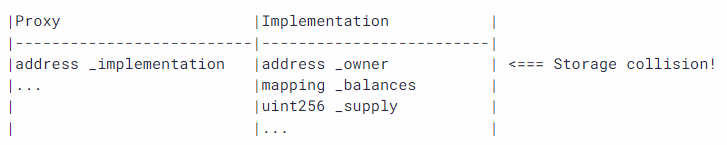
\includegraphics[width=\textwidth,height=6cm,keepaspectratio=true]{collision_1.png}
   \caption{
       A storage collision between proxy and logic data \cite{zeppelin_proxy}
   }
\end{figure}


Another example from OpenZeppelin shows how a collision happens when a contract upgrade is not performed correctly.
The order of variables inside the source code must be preserved.
If not done correctly, the already saved data clashes with the new field saved at that particular slot.
\begin{figure}[htpb]
   \centering
   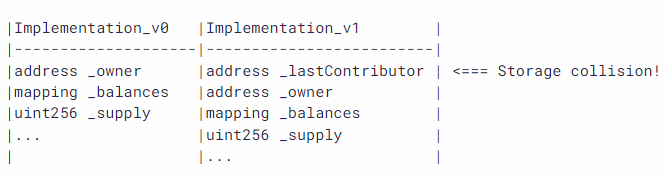
\includegraphics[width=\textwidth,height=6cm,keepaspectratio=true]{version_collision.png}
   \caption{
       A storage collision after a contract update \cite{zeppelin_proxy}
   }
\end{figure}

In addition to storage collisions, there are also function clashes.
They are described as two functions named the same or sharing the same 4-byte code identifier, resulting in a collision.
A transparent proxy solves this issue by picking the function based on the address of the function caller.

\begin{quote}
\centering 
   \textit{If the caller is the admin of the proxy (the address with rights to upgrade the proxy), then the proxy will not delegate any calls and will only answer any messages it understands.}
   \textit{If the caller has any other address, it will always delegate a call, whether it matches one of the proxy's functions.} \cite{zeppelin_proxy}
\end{quote}


\subsection{Problem: Blockchain Scalability}
Blockchains' scalability issues come with using blockchains to store external data or execute smart contract logic.
Every state-changing action requires a transaction, while all transactions compete for block space with fees.
The Bitcoin blockchain processes about seven transactions per second, which is neither suitable as a protocol to use for daily transactions nor would that grant
sufficient speed for code execution. Ethereum already has a block time of a few seconds compared to Bitcoin's block time of ten minutes.
Yang, Long, Xu, and Peng analyzed the scalability problem of blockchains in \cite{blockchain_scalability} and named potential solutions.

One of these solutions is called \textbf{Sharding}. 
A concept initially designed to split large databases into smaller ones to distribute the workload and enhance efficiency.
In the blockchain context, smaller chains, called shards, produce blocks that are appended to the main chain.
While this process allows for faster transaction speeds and improved network performance, some drawbacks could lead to potential security problems.
One of them is a Single Shard Takeover Attack. 
Taking over the Bitcoin blockchain requires an attacker to have more processing power than the rest of the network.
However, taking over a shard requires a percentage of the original amount.
Besides, managing the shards and efficiently balancing the workloads requires complex code that could lead to new vulnerabilities and bugs. \cite{sharding_binance}

Another concept is the use of off-chain payment networks.
Instead of changing the blockchain or its consensus rules, the use of the protocol is changed.
Accordingly, the underlying blockchain serves as a settlement base layer.
Smaller transactions are performed in the payment network.
The settlement is done by publishing one transaction containing billions of off-chain transactions.
One example of such a network is the \textbf{Bitcoin Lightning network} \cite{poon2016}.
It creates multi-signature wallets between two parties that serve as payment channels.
Transactions between these two entities are not tracked on-chain. 
Instead, the settlement transaction is done when closing the channel. 
As a result, network channels can be used to route payments through the network.
If Alice has a payment channel with Bob and Bob has a channel with Tom, Alice can send funds to Tom.
However, the network also comes with some drawbacks.
Since two parties share a payment channel, users are advised to keep their lightning node online to prevent fraudulent behavior.
Else, it would be possible to steal funds from the channel.
Besides, the network needs liquidity to route payments. 
If Alice wants to send 0.5 bitcoin to Tom, but the channel between Tom and Bob does not have 0.5 bitcoin for routing, it cannot be done.
The only way to transfer liquidity into the network is by issuing main-chain transactions to lock the coins into a payment channel.

Besides the Lightning network, there are other implementations for other blockchains, further described in \cite{blockchain_scalability}.
While there are more solutions for the scalability problem, more scalability always comes with drawbacks.
This consequence is called \textbf{blockchain trilemma} \cite{blockchain_trilemma}, meaning the trade-off between decentralization, security, and scalability.
Bitcoin was designed concerning decentralization and security, resulting in a low transaction speed and, thus, less scalability.
This design choice serves the narrative of a blockchain being a secure payment network without relying on a trusted third party.
As a result, using blockchains to store data or execute code is always limited by blockchain technology.
The chain would lose its initial purpose if a scaling solution leading to less decentralization or security problems were used.
Hence, using blockchains over centralized services will always be less efficient.

\section{Opportunities of Smart Contracts for Software Engineering}
Besides these drawbacks, there are also opportunities.
Before evaluating these arguments, it is crucial to note that every argument for blockchains and smart contract usage should exclude any oracles or third parties.
Otherwise, the blockchain would lose the decentralization features it was made for, while the software engineering problems would stay.
When implementing solutions or concepts using smart contracts, the Oracle problem is the most crucial question to ask.
Even if a full game or program is implemented using only smart contracts, the programmer might always have special administrative rights to control certain contract parts.
For example, the administrator could issue virtual items with admin functions instead of using the normal contract functions. Alternatively, some variables of the contract could be changed.
If not fully solved or even addressed, centralized services will always be a better design choice to implement data or code logic.

\subsection{Opportunity: Code Transparency}
Due to the nature of public blockchains, all data is available for everyone at any time.
Hence, all smart contracts and their byte code are public as well.
This transparency could be used as a feature to implement specific game program codes into the chain, such as random number generators for loot drops or crucial game mechanics.
However, it is not guaranteed that any game uses these contracts.
Furthermore, the company producing a game could change its source code and not use smart contracts anymore.
Thus, users again face the oracle problem.
However, the argument might be valid if the whole game is programmed with smart contracts, with all the software engineering drawbacks.
Games that use this approach can only implement a few game mechanics due to the scalability issues. \cite{8848111}

\subsection{Opportunity: Code Reusability}
Since anyone can execute smart contracts, different games can use them simultaneously.
Character stats or virtual items could be beneficial in different games. 
In addition, if more than one game uses the virtual item, the value is not dependent on only one-third party.
While this argument does not solve the oracle problem, it at least distributes the counterparty risk to many third parties. \cite{8848111}

Besides, using existing code and a functioning blockchain reduces the workload.
With blockchains, an existing infrastructure that requires neither maintenance nor running costs can be used.
When game items or logic are already implemented on the chain, games can adopt them and connect their product to an existing ecosystem. 
However, the oracle problem will always be a part of these solutions, which results in the question of whether centralized services would also work
to achieve the same outcome.